%!TEX program = xelatex

\documentclass[compress]{beamer}


\usepackage{pgfpages}

\mode<handout>{%
    \pgfpagesuselayout{4 on 1}[a4paper]
    \setbeameroption{show notes}
}
%--------------------------------------------------------------------------
% Common packages
%--------------------------------------------------------------------------

\definecolor{links}{HTML}{663000}
\hypersetup{colorlinks,linkcolor=,urlcolor=links}

\usepackage[english]{babel}
\usepackage{pgfpages} % required for notes on second screen
\usepackage{graphicx}

\usepackage{multicol}

\usepackage{tabularx,ragged2e}
\usepackage{booktabs}
\usepackage{pseudocode}

\setlength{\emergencystretch}{3em}  % prevent overfull lines

\usetheme{hri}
\usetikzlibrary{shapes.geometric}
\usetikzlibrary{svg.path}

% Display the navigation bullet even without subsections
\usepackage{remreset}% tiny package containing just the \@removefromreset command
\makeatletter
\@removefromreset{subsection}{section}
\makeatother
\setcounter{subsection}{1}

\makeatletter
\let\beamer@writeslidentry@miniframeson=\beamer@writeslidentry
\def\beamer@writeslidentry@miniframesoff{%
  \expandafter\beamer@ifempty\expandafter{\beamer@framestartpage}{}% does not happen normally
  {%else
    % removed \addtocontents commands
    \clearpage\beamer@notesactions%
  }
}
\newcommand*{\miniframeson}{\let\beamer@writeslidentry=\beamer@writeslidentry@miniframeson}
\newcommand*{\miniframesoff}{\let\beamer@writeslidentry=\beamer@writeslidentry@miniframesoff}
\makeatother



\newcommand{\source}[2]{{\tiny\it Source: \href{#1}{#2}}}

\usepackage{tikz}
\usetikzlibrary{mindmap,backgrounds,positioning,calc,patterns}

\graphicspath{{figs/}}

\title{Symbolic Reasoning for HRI}
\subtitle{~}
\date{}
\author{Séverin Lemaignan}
\institute{{\bf Bristol Robotics Lab}\\University of the West of England}


% for model of anthopomorphism
\newcommand{\IPA}{{$\mathcal{A}_0$~}}
\newcommand{\SLA}{{$\mathcal{A}_\infty$~}}
\newcommand{\sla}{{\mathcal{A}_\infty}}
\newcommand{\AntMax}{{$\mathcal{A}_{max}$~}}
\newcommand{\antMax}{{\mathcal{A}_{max}}}

\newcommand{\chatN}[1]{{\footnotesize \textsf{#1}}}

% for HATP plans
\newcommand{\hatpaction}[3]{#1\\\textsf{\scriptsize #2,}\\\textsf{\scriptsize #3}}
\newcommand{\stmt}[1]{{\footnotesize \tt  #1}}

% for mutual modelling
\newcommand{\Mmodel}[3]{{\mathcal{M}(#1, #2, #3)}}
\newcommand{\model}[3]{{$\mathcal{M}(#1, #2, #3)$}}
\newcommand{\Model}[3]{{$\mathcal{M}^{\circ}(#1, #2, #3)$}}

% typeset logical concept
\newcommand{\concept}[1]{{\scriptsize \texttt{#1}}}

\begin{document}

\miniframesoff

\licenseframe{github.com/severin-lemaignan/lecture-hri-symbolic-reasoning}

\maketitle

\miniframeson

\begin{frame}{In this lecture}

\begin{itemize}
    \item<1-> Lecture on speech: NLP down to syntax parsing
    \item<2-> Today: \textbf{meaning} (both semantics and pragmatics)

    \begin{itemize}
        \item<4-> How to attach \emph{meaning} to perceptions \& natural language?
        \item<4-> What are ontologies?
        \item<4-> How is `meaning' represented and used within the robot?
        \item<4-> How does it relate to \emph{mental models}?
    \end{itemize}

        \onslide<3->{

\begin{exampleblock}{Semantics vs Pragmatics}
    \emph{Semantics} is the (conventional) meaning attached to words and
    sentences; \emph{Pragmatics} study the actual meaning coming out of the
    context: who speaks? how they speak? what common knowledge between the
    speaker and the listener? what is the situation? etc.
\end{exampleblock}


        }
\end{itemize}

\end{frame}

\section*{Introduction}


\imageframe{pr2-baby-3}


\begin{frame}[plain]

    \centering
    {\bf Situated dialogue} effectively evidences the challenges

    \begin{columns}
        \begin{column}{0.5\linewidth}
            How can the robot make sense of and act upon a sequence of letters
            like:
            \vspace{2em}

            \bf
            ``Can you give me that book?''
        \end{column}
        \begin{column}{0.5\linewidth}
            \begin{center}
                \includegraphics[width=\linewidth]{pr2-baby-3}
            \end{center}
        \end{column}
    \end{columns}

\end{frame}


{\paper{Harnad, \emph{The Symbolic Grounding Problem}, 1990}

\begin{frame}{The Symbol Grounding Problem}
    \centering
    \only<1>{
    \Large How to attach meaning to a symbol?
    }

    \normalsize

    \only<2>{
        Google Translate translates French ``\emph{Il pleut comme vache qui
        pissent}'' into English ``\emph{It's raining cats and dogs}''.
        
        ...no peeing cow?? Does Google Translate \emph{understand} French and/or
        English?
    }

    \only<3>{

        The mind as a computer:\\
        \emph{functionalism} \& Searle's \textbf{Chinese Room Argument}

        \begin{center}
            \includegraphics[width=0.8\linewidth]{chinese-room}
        \end{center}


        \href{https://en.wikipedia.org/wiki/Chinese_room}{Read more on Wikipedia}

    }
    \only<4>{

        {\Large How to attach meaning to a symbol?}

        Is it possible at all?
        Is it actually necessary?

    }
    \only<5>{
        \Large
        \textbf{Embodiement} is part of the answer. In robotics, we talk of
        \textbf{Situated AI}.
    }


\end{frame}

}

%%%%%%%%%%%%%%%%%%%%%%%%%%%%%%%%%%%%%%%%%%%%%%%%%%%%%%%%
\section[Symbolic cognition]{Situated, Grounded, Symbolic social cognition}


{
    \paper{Lemaignan et al., \emph{Artificial Cognition for Social Human-Robot
    Interaction: An Implementation}, Artifical Intelligence, 2017}
\begin{frame}{Situation Assessment}
        \centering
        \video{0.9\textwidth}{videos/model3d.webm}\\

\end{frame}
}

\begin{frame}{Visual Perspective taking}

        \centering
        \includegraphics[width=0.8\textwidth]{spark_vert.pdf}

\end{frame}

{
    \paper{Lemaignan et al., \emph{Artificial Cognition for Social Human-Robot
    Interaction: An Implementation}, Artifical Intelligence, 2016}
\begin{frame}{}
        \centering
        \scriptsize

        \begin{tabular}{p{1.5cm}lp{2cm}}
            Subject & Predicate  & Object  \\ 
            \hline
            \concept{Location} & \concept{isAt}  &  \concept{Location}  \\ 
                               &  $\rightarrow$ \concept{isOn}  &   \\ 
                               &  $\rightarrow$ \concept{isIn}  &   \\ 
                               &  $\rightarrow$ \concept{isNextTo}  &   \\ 

            \concept{Location}  & \concept{isAbove}  &  \concept{Location} \\ 
            \concept{Location}  & \concept{isBelow}  & \concept{Location} \\
            \hline
            \concept{Location}  & \concept{hasRelativePosition}  & \concept{Location}  \\ 
                                   & 	$\rightarrow$ \concept{behind} & \\ 
                                      &  $\rightarrow$ \concept{inFrontOf}  & \\ 
                                         &  $\rightarrow$ \concept{leftOf}  &  \\ 
                                            &  $\rightarrow$ \concept{rightOf}  & 	 \\ 
            \concept{Object}  & \concept{farFrom}  &  \concept{Agent} \\ 
            \concept{Object}  & \concept{near}  &  \concept{Agent} \\

            \hline
            \concept{Agent}  & \concept{looksAt}  & \concept{SpatialThing} \\
            \concept{Agent}  & \concept{sees}  &  \concept{SpatialThing}  \\ 
            \concept{SpatialThing}  & \concept{isInFieldOfView}  & \concept{xsd:boolean}  \\ 
            \concept{Agent}  & \concept{pointsAt}  & \concept{SpatialThing} \\ 
            \concept{Agent}  & \concept{focusesOn}  &  \concept{SpatialThing}  \\ 
            \concept{Agent} & \concept{seesWithHeadMovement} &  \concept{SpatialThing} \\
            \concept{Agent} & \concept{canReach} &  \concept{Object} \\ 

        \end{tabular}

\end{frame}
}

\begin{frame}{Statement, beliefs}
    \centering

    \stmt{\normalsize human\_1 sees teddybear}

    \pause

    \Large
    A \textbf{statement} is a true proposition (in a given model)
    \pause
    $\equiv$ \textbf{belief}
    \pause

    \stmt{\normalsize teddybear type Toy}

    \pause

    \stmt{\normalsize teddybear isOn table\_1}

    \pause

    \stmt{\normalsize human\_1 hates robot\_1} (in the human's model only!)

\end{frame}


\begin{frame}{Statement, beliefs (2)}
    \centering
    \Large

    \stmt{\normalsize human\_1 sees teddybear}


    Triplet $\langle S, P, O \rangle$: subject, predicate, object

    \pause

    $P$ is a predicate of \textbf{arity} 2: $P(S, O)$

    \vspace{1em}
    \begin{overlayarea}{\textwidth}{4cm}

        \normalsize

    \only<3>{
    Some logic language (like Prolog) allows arbitrary arities:

    \stmt{\normalsize give(robot\_1, human\_1, teddybear)}
    }

    \only<4>{

    Many do not (like the OWL language). In this case, \textbf{reification}:

    \stmt{give\_act\_1 type Give} 

    \stmt{give\_act\_1 performedBy robot\_1} 

    \stmt{give\_act\_1 receivedBy human\_1} 

    \stmt{give\_act\_1 actsOnObject teddybear}

    }

    \end{overlayarea}

\end{frame}

\begin{frame}{Towards ontologies}

    \only<1>{
        The robot's newly acquired beliefs typically have to be \textbf{anchored} in
        pre-existing knowledge.

        $\rightarrow$ We usually endow the robot with \textbf{background knowledge} (also
        known as \textbf{common-sense knowledge}) with statements like:

        \stmt{Object rdfs:subclassOf PhysicalThing}

        \stmt{Location rdfs:subclassOf SpatialThing}
    }

    \only<2>{

    \centering
    \begin{figure}

        \resizebox{0.9\paperwidth}{!}{%
            \begin{tikzpicture}[
                    >=latex,
                    every edge/.style={<-, draw, very thick},
                    every node/.style={draw, font=\sf, node distance=0.5, rounded corners,
                align=center, inner sep=5pt,fill=hriSec2Dark!50}]

                \node[fill=hriSec2Comp!50] (thing) {\bf thing};
                \node [fill=hriSec3CompDark!50, node distance=1.8, below left=of thing](sthing) {spatial thing} edge (thing);
                \node [fill=hriSec3CompDark!50, above left=of sthing] {posture} edge (sthing);
                \node [fill=hriSec3CompDark!50, left=of sthing] {shape} edge (sthing);
                \node [fill=hriSec3CompDark!50, below=of sthing] (location) {location} edge (sthing);
                \node [fill=hriSec3CompDark!50, below right=of location] {zone} edge (location);
                \node [fill=hriSec3CompDark!50, below left=of location] (set) {spatial enduring thing} edge (location);
                \node [fill=hriSec3CompDark!50, below right=of set] {obstacle} edge (set);
                \node [fill=hriSec3CompDark!50, below left=of set] {opening} edge (set);
                \node [fill=hriSec3CompDark!50, below=1 of set] {partially tangible thing} edge (set);
                \node [fill=hriSec3CompDark!50, above left=of set] {place} edge (set);

                \node [node distance=1, below right=of thing] (tthing) {temporal thing} edge (thing);
                \node [below=of tthing] (tte) {thing with temporal extent} edge (tthing);
                \node [below right=of tte] {time interval} edge (tte);
                \node [below=1 of tte] (sit) {situation} edge (tte);
                \node [below right=of sit] (evt) {event} edge (sit);
                \node [below right=of evt] (act) {action} edge (evt);
                \node [below=of act] {purposeful action} edge (act);
                \node [below left=of sit] {static situation} edge (sit);

            \end{tikzpicture}
            }
    \end{figure}

    \large
    Example of an \textbf{upper ontology}

    }

\end{frame}


\begin{frame}{Ontologies}


    \centering
    \Large
     An \textbf{ontology} encompasses a representation, formal naming, and definition of the categories,
     properties, and relations between the concepts, data, and entities that
     substantiate one, many, or all domains.

     \normalsize

     \onslide<2->{(also known as a \textbf{knowledge graph})}

     \onslide<3>{Ontologies often have close relationships with \textbf{first-order logic
     (FOL)}
     -- more about that later.}

\end{frame}

\begin{frame}{Ontologies}

    \begin{itemize}
        \item \textbf{T-box} statements: the \emph{conceptualisation} of the
            domain, for instance in terms of \emph{categories} (classes): \stmt{Dog
            rdfs:subClassOf Animal}

        \item \textbf{A-box} statements: (T-box compliant) statements about
            \emph{individuals} (instances) in the ontology: \stmt{SPOT rdf:type Dog}

    \end{itemize}

    \pause

    Ontologies are represented using a \textbf{knowledge description language}.
    The \textbf{Web Ontology Langage (OWL)} is a common choice that uses a
    XML encoding.
\end{frame}

\begin{frame}{Online instanciation}

    \begin{columns}
        \begin{column}{0.4\linewidth}
        \centering
        \includegraphics[width=\linewidth]{human-perspective-small}
             
        \end{column}
        \begin{column}{0.6\linewidth}
        
        \begin{figure}

        \resizebox{\columnwidth}{!}{%
        \begin{tikzpicture}[
            yscale=1.3,
            >=latex,
            every edge/.style={<-, draw, very thick},
            every node/.style={draw, font=\sf, node distance=0.5, rounded corners,
            align=center, inner sep=5pt,fill=hriSec2Dark!50},
            classof/.style={<-, draw=black!60, dashed},
            property/.style={<-, draw=hriSec2Comp},
            propname/.style={above, draw=none, fill=none, font=\tt, inner sep=2pt},
            instance/.style={draw=hriSec1Dark, font=\sf, node distance=0.5, rounded corners,
        align=center, inner sep=5pt, fill=none}]

            \node[fill=hriSec2Comp!50] (thing) {\textbf{thing}};
            \node [fill=hriSec3CompDark!50, node distance=1.8, below left=of
            thing](sthing) {place} edge[dashed] (thing);
            \node [fill=hriSec3CompDark!50, below left=of sthing] (agent) {agent} edge (sthing);
                \node [fill=hriSec3CompDark!50, below=of sthing] (artifact) {artifact} edge (sthing);
                \node [fill=hriSec3CompDark!50, below right=of sthing] (location) {physical
                support} edge (sthing);
                \node [fill=hriSec3CompDark!50, below right=of artifact] (table) {table}
                    edge (location) edge (artifact);


            \node [node distance=1, below right=of thing] (tthing) {temporal thing} edge (thing);
                \node [below right=of tthing] (evt) {event} edge[dashed] (tthing);
                            \node [below right=of evt] (act) {action} edge (evt);

        \uncover<2->{
        \draw[dotted, thick] (-8,-3.8) -- +(16, 0);

        \node [instance, below=3 of agent] (human) {human\_1} edge[classof, bend left] (agent);
        \node [instance, above left=of human] (human2) {human\_2} edge[classof, bend left] (agent);
        \node [instance, above right=of human, anchor=south] (robot) {myself} edge[classof, bend left] (agent);
        \node [instance, right=of human, anchor=north west] (book)
            {harry\_potter}
        edge[classof] (artifact);
        \node [instance, right=2 of robot] (ikea) {ikea\_table} edge[classof, bend
        right] (table);
        \node [instance, right=2 of book] (brown) {brown} edge[property] node[propname] {hasColor} (book);


        }
        \uncover<3>{
        \draw[dotted, thick] (-8,-6.2) -- +(16, 0);

        \node [instance, below=5 of act] (moving) {move\_act\_42} edge[classof] (act);
        \path (moving.west) edge [property, out=180, in=-80, looseness=1] node[propname,below] {currentlyPerforms} (human.230);
        \path (human.280) edge [property, out=-80, in=-90, looseness=3.5] node[propname,right] {looksAt} (robot.south);
        \path (ikea.south) edge [property, out=-90, in=-80, looseness=2.5] node[propname, auto] {isOn} (book.320);
        }
        \end{tikzpicture}
        }

        \end{figure}

       \end{column}
    \end{columns}




\end{frame}
%}

%%%%%%%%%%%%%%%%%%%%%%%%%%%%%%%%%%%%%%%%%%%%%%%%%%%%%%%%
%

\begin{frame}[plain]

    \centering
    \Large

    Back to our initial example:

    \textbf{Give me that book!}

\end{frame}

{
\paper{Lemaignan et al. \emph{Grounding the Interaction: Anchoring
Situated Discourse in Everyday HRI} -- Intl. J. of Social Robotics 2011}

\begin{frame}{Dialogue Grounding}
    \begin{figure}
        \centering

        \resizebox{0.4\paperwidth}{!}{%


            \begin{tikzpicture}[
                    >=latex,
                every edge/.style={draw, very thick},
                skill/.style={draw, rounded corners, align=center, inner sep=5pt, fill=black!20},
                label/.style={midway, align=center, font=\scriptsize, above},
                subpart/.style={rounded corners, draw, align=center, font=\scriptsize, fill opacity=0.5, text opacity=1, fill=white!50}]

            %%% PARSING

            \node at (0,0)[skill, fill=hriSec3CompDark!50] (prepro) {Pre-processing};
                \node [left=0.7 of prepro] (input) {\textbf{Input}};
                \path (input) edge [->] (prepro);

                %\path (spark.100) edge [->, bend right] node[label] {symbolic \\ facts} (oro);
                \node [below =0.4 of prepro, skill, fill=hriSec3CompDark!50] (parsing) {Parsing};
                \path (prepro) edge [->] (parsing);

                \coordinate (base-onto) at (4,0);

                %%% RESOLUTION
                \uncover<2->{
                    \node [below=0.4 of parsing, skill, fill=hriSec3!50, minimum height=4cm, minimum width=5cm] (resolution) {};
                \node [subpart, below=0.2 of resolution.115] (pron) {Pronouns \& \\ anaphora resolution};
                \node [subpart, below=0.2 of pron] (noun) {Noun phrase \\ resolution};
                \node [subpart, right=0.3 of noun, anchor=north west] (discr) {Discrimination};
                \node [subpart, below=0.2 of noun] (verb) {Verbal phrase \\ resolution};
                \node [subpart, cylinder, shape border rotate=90, aspect=0.5, below=0.2 of discr] (actions) {Actions};
                \path (pron) edge [->] (noun);
                \path (noun) edge [->] (discr);
                \path (noun) edge [->] (verb);
                \path (verb) edge [dashed, <->] (actions);
                \path (pron) edge [dashed, <->] node[label] {queries} (pron -| base-onto);
                \path (noun.20) edge [dashed, <->] node[label] {queries} (noun.20 -| base-onto);
                \path (discr) edge [<->] (discr -| base-onto);

                \node [left=0.2 of resolution.west, rotate=90, anchor=south] {Resolution};
                \path (parsing) edge [->] (pron);
            }

            %%% INTERPRETATION
                \uncover<3->{
                    \node [skill, below=0.4 of resolution,minimum width=5cm, minimum height=3cm] (interp) {};
                \node [subpart, below=0.2 of interp.north] (content) {Content analysis};
                \node [below=0.6 of content.south west, subpart] (question) {Question \\ handler};
                \node [below=0.6 of content.south east, subpart] (stat) {Statement \\ builder};
                \path (content) edge [->] node[label, left] {question} (question);
                \path (content) edge [->] node [label, right] {goal | statement} (stat);
                \path (stat) edge [->] node [label] {asserts} (stat -| base-onto);

                \node [left=0.2 of interp.west, rotate=90, anchor=south] {Interpretation};

                \path (verb) edge [->] (content);
                \path (question) edge [dashed, bend right, <->] node[label] {queries} (question.south -| base-onto);
            }

            %%% ONTOLOGY
                \uncover<2->{
                    \node at (resolution.north -| base-onto) [rotate=-90, skill, minimum height=2cm, minimum width=7cm, fill=hriSec3!50, anchor=south west] (onto) {Ontology};

                }

            %%% VERBALIZATION
            \uncover<4->{
                \node [below=0.7 of interp, skill, fill=hriSec2Dark!50] (verb) {Verbalization};
            \path (question) edge [->] (verb);
            \path (stat) edge [->] (verb);
            \path (discr.south east) edge [black!50, dashed, bend left, <->] (verb.north east);
            \node [right=0.7 of verb] (output) {\textbf{Output}};
            \path (verb) edge [->] (output);
        }
        \end{tikzpicture}
        }
    \end{figure}

\end{frame}
}


{
\paper{Lemaignan et al. \emph{Grounding the Interaction: Anchoring
Situated Discourse in Everyday HRI} Intl. J. of Social Robotics 2011}
\begin{frame}{Dialogue Grounding}
    \centering


    \begin{columns}
        \begin{column}{0.65\linewidth}

    \centering
    \vspace*{2em}
    {\bf ``Give me the book on the table''}\\

    \uncover<2-> {
        $\downarrow$\\
        {\tt me} $\rightarrow$ {\tt human\_1} \\
        find({\tt\scriptsize ?obj type Table}) $\rightarrow$ {\tt ikea\_table} \\
        find({\tt\scriptsize ?obj type Book, ?obj isOn ikea\_table})
        $\rightarrow$ {\tt harry\_potter} \\
    }

    \uncover<3-> {
        $\downarrow$\\
        { \tt \small
            \textbf{human\_1} desires \textbf{give\_act\_1}, \\
            \textbf{give\_act\_1} type \textbf{Give}, \\
            \textbf{give\_act\_1} performedBy \textbf{myself}, \\
            \textbf{give\_act\_1} actsOnObject \textbf{harry\_potter}, \\
            \textbf{give\_act\_1} receivedBy \textbf{human\_1} \\
        }
    }
            
        \end{column}
        \begin{column}{0.35\linewidth}
         \resizebox{\linewidth}{!}{%
 
 
             \begin{tikzpicture}[
                     >=latex,
                 every edge/.style={draw, very thick},
                 skill/.style={draw, rounded corners, align=center, inner sep=5pt, fill=black!20},
                 label/.style={midway, align=center, font=\scriptsize, above},
                 subpart/.style={rounded corners, draw, align=center, font=\scriptsize, fill opacity=0.5, text opacity=1, fill=white!50}]
 
             %%% PARSING
 
             \node at (0,0)[skill, fill=hriSec3CompDark!50] (prepro) {Pre-processing};
                 \node [left=0.7 of prepro] (input) {\textbf{Input}};
                 \path (input) edge [->] (prepro);
 
                 %\path (spark.100) edge [->, bend right] node[label] {symbolic \\ facts} (oro);
                 \node [below =0.4 of prepro, skill, fill=hriSec3CompDark!50] (parsing) {Parsing};
                 \path (prepro) edge [->] (parsing);
 
                 \coordinate (base-onto) at (4,0);
 
                 %%% RESOLUTION
                     \node [below=0.4 of parsing, skill, fill=hriSec3!50, minimum height=4cm, minimum width=5cm] (resolution) {};
                 \node [subpart, below=0.2 of resolution.115] (pron) {Pronouns \& \\ anaphora resolution};
                 \node [subpart, below=0.2 of pron] (noun) {Noun phrase \\ resolution};
                 \node [subpart, right=0.3 of noun, anchor=north west] (discr) {Discrimination};
                 \node [subpart, below=0.2 of noun] (verb) {Verbal phrase \\ resolution};
                 \node [subpart, cylinder, shape border rotate=90, aspect=0.5, below=0.2 of discr] (actions) {Actions};
                 \path (pron) edge [->] (noun);
                 \path (noun) edge [->] (discr);
                 \path (noun) edge [->] (verb);
                 \path (verb) edge [dashed, <->] (actions);
                 \path (pron) edge [dashed, <->] node[label] {queries} (pron -| base-onto);
                 \path (noun.20) edge [dashed, <->] node[label] {queries} (noun.20 -| base-onto);
                 \path (discr) edge [<->] (discr -| base-onto);
 
                 \node [left=0.2 of resolution.west, rotate=90, anchor=south] {Resolution};
                 \path (parsing) edge [->] (pron);
 
             %%% INTERPRETATION
                     \node [skill, below=0.4 of resolution,minimum width=5cm, minimum height=3cm] (interp) {};
                 \node [subpart, below=0.2 of interp.north] (content) {Content analysis};
                 \node [below=0.6 of content.south west, subpart] (question) {Question \\ handler};
                 \node [below=0.6 of content.south east, subpart] (stat) {Statement \\ builder};
                 \path (content) edge [->] node[label, left] {question} (question);
                 \path (content) edge [->] node [label, right] {goal | statement} (stat);
                 \path (stat) edge [->] node [label] {asserts} (stat -| base-onto);
 
                 \node [left=0.2 of interp.west, rotate=90, anchor=south] {Interpretation};
 
                 \path (verb) edge [->] (content);
                 \path (question) edge [dashed, bend right, <->] node[label] {queries} (question.south -| base-onto);
 
             %%% ONTOLOGY
                     \node at (resolution.north -| base-onto) [rotate=-90, skill, minimum height=2cm, minimum width=7cm, fill=hriSec3!50, anchor=south west] (onto) {Ontology};
 
 
             %%% VERBALIZATION
                 \node [below=0.7 of interp, skill, fill=hriSec2Dark!50] (verb) {Verbalization};
             \path (question) edge [->] (verb);
             \path (stat) edge [->] (verb);
             \path (discr.south east) edge [black!50, dashed, bend left, <->] (verb.north east);
             \node [right=0.7 of verb] (output) {\textbf{Output}};
             \path (verb) edge [->] (output);
         \end{tikzpicture}
         }

        \end{column}
    \end{columns}


\end{frame}
}
%
%%%%%%%%%%%%%%%%%%%%%%%%%%%%%%%%%%%%%%%%%%%%%%%%%%%%%%%%%

{
    \paper{Lemaignan et al., {\bf Artificial Cognition for Social Human-Robot
    Interaction: An Implementation}, Artifical Intelligence, 2017}
\begin{frame}{Multi-modal interaction}

    \begin{columns}
        \begin{column}{0.4\linewidth}
        \centering
        \includegraphics[width=\linewidth]{human-perspective-small}
             
        \end{column}
        \begin{column}{0.6\linewidth}
        
    \centering
    What about

    {\bf ``Give me \emph{that} book''}?

     \footnotesize
    (or even: {\bf ``Give me \emph{that}!''})

       \end{column}
    \end{columns}




\end{frame}
}

%\videoframe[0.56]{videos/this_box.webm}
\videoframe[0.56]{videos/this_box.mp4?autostart&start=1}

\begin{frame}{Example of first-order logic reasoning}
    \centering

    \vspace*{2em}
    ``Where is the other tape?''\\
    $\downarrow$\\
    find({\tt\scriptsize ?obj isAt ?loc, ?obj type VideoTape, ?obj differentFrom WALL\_E})

    \pause

    \vspace*{2em}
    Symbolic approaches effective at dealing with this kind of constraints

\end{frame}

\begin{frame}{Interaction example: I Spy With My Little Eye}

    \centering
    \only<1>{

        \includegraphics[width=0.45\textwidth]{spy-game-real}
        \includegraphics[width=0.45\textwidth]{spy-game-mhp}
    }
    \only<2>{
        \resizebox{\textwidth}{!}{
        \begin{tikzpicture}[
                    >=latex,
                    edge from parent/.style={->, draw, very thick},
                    level 1/.style={sibling distance=50mm},
                    level 2/.style={thin,sibling distance=40mm},
                    level 3/.style={thin, sibling distance=15mm},
                    level 4/.style={thin, sibling distance=25mm},
                    every node/.style={draw, font=\sf, rounded corners,
                        align=center, inner sep=5pt,fill=hriSec3CompDark!50},
                    property/.style={->, draw=hriSec2Comp},
                    propname/.style={above, draw=none, fill=none, font=\tt, inner sep=2pt},
                    instance/.style={draw=hriSec1Dark,
                    font=\sf, node distance=0.5, rounded corners,
                        align=center, inner sep=5pt, fill=white}
            ]
            \node {Place} 
            child {node {Agent}
                child {node[instance] (human) {\footnotesize human}}
            }
            child {node {Artifact}
                child {node {Tableware}
                child {node {Bottle}
                    child {node[instance] (bluebottle) {\footnotesize blue-bottle}}
                    child {node[instance] (yellowbottle) {\footnotesize yellow-bottle}}
                    child {node[instance] {\footnotesize orange-bottle}}
                }
                child {node {Cup}}
                }
                child {node {Furniture}
                child {node {Table}}
                child {node {Chair}}
                child {node {Shelf}}}
            };
            
            \path (human) edge [property] node[propname,auto] {sees} (bluebottle);
            \path (human) edge [property] (yellowbottle);
        \end{tikzpicture}
    }

    }
    \only<3>{
        \small
        \begin{tabular}{r|p{0.7\columnwidth}}
            \chatN{human} & It is a tableware.\\
            \chatN{robot} & \emph{[retrieves possible objects: blue-bottle, yellow-bottle, orange-bottle, cup-with-handle]} \\
                & \emph{[keeps human-visible objects: blue-bottle, yellow-bottle, cup-with-handle]}\\
                & \emph{[obtains discriminants: type, color.]}\\
                & Which type of object is: bottle or cup? \\
            \chatN{human} & Bottle.\\
            \chatN{robot} & \emph{[obtains possible objects: blue-bottle, yellow-bottle.]}\\
                & \emph{[obtains discriminants: color.]}\\
                & What color the object is: blue or yellow?\\
            \chatN{human} & Blue.\\
            \chatN{robot} & \emph{[obtains possible objects: blue-bottle.]}\\
                & The object is the blue-bottle!	
        \end{tabular}\\


    }

\end{frame}



%%%%%%%%%%%%%%%%%%%%%%%%%%%%%%%%%%%%%%%%%%%%%%%%%%%%%%%%%
%
\section[Theory of Mind]{One step further: Theory of Mind}
%
%%%%%%%%%%%%%%%%%%%%%%%%%%%%%%%%%%%%%%%%%%%%%%%%%%%%%%%%%
{ \paper{Wimmer and Perner, {\bf Beliefs about beliefs: Representation and
constraining function [...]}, Cognition, 1983]%\newline
%        [Lemaignan, Dillenbourg {\bf Mutual Modelling in Robotics: Inspirations
%        for the Next Steps} -- HRI 2015
}
\begin{frame}{1st order ToM: the False-Belief Experiment}

        \begin{center} 
            \includegraphics[width=0.7\textwidth]{sally_ann.pdf}
        \end{center}
\end{frame}
}

\begin{frame}[plain]

    \begin{center}
        \includegraphics[width=0.8\linewidth]{videos/this_box_thumb}

        What if I ask for the video tape in the box, but the robot previously
        moved it somewhere else?


    \pause

        {\bf False-belief situation}
    \end{center}
\end{frame}

%%%%%%%%%%%%%%%%%%%%%%%%%%%%%%%%%%%%%%%%%%%%%%%%%%%%%%%%%

\begin{frame}{Parallel Models: towards theory of mind}
        \begin{multicols}{2}
            \begin{figure}
                \resizebox{0.4\textwidth}{!}{
                    \begin{tikzpicture}[
                        >=latex,
                        every edge/.style={<-, draw, very thick},
                        every node/.style={draw, font=\sf, node distance=0.5, rounded corners,
                                        align=center, inner sep=5pt,fill=hriSec2Dark!50},
                        classof/.style={<-, draw=black!60, dashed},
                        property/.style={<-, draw=hriSec2Comp},
                        propname/.style={above, draw=none, fill=none, font=\tt, inner sep=2pt},
                        instance/.style={draw=hriSec1Dark, font=\sf, node distance=0.5, rounded corners,
                        align=center, inner sep=5pt, fill=white}]

                    \node[fill=hriSec2Comp!50] (thing) {\textbf{thing}};
                    \node [fill=hriSec3CompDark!50, node distance=1.8, below left=of thing](sthing) {place} edge[dashed] (thing);
                    \node [fill=hriSec3CompDark!50, below left=of sthing] (agent) {agent} edge (sthing);
                        \node [fill=hriSec3CompDark!50, below=of sthing] (artifact) {artifact} edge (sthing);
                        \node [fill=hriSec3CompDark!50, below right=of sthing] (location) {physical
                        support} edge (sthing);
                        \node [fill=hriSec3CompDark!50, below right=of artifact] (table) {table}
                            edge (location) edge (artifact);


                    \node [node distance=1, below right=of thing] (tthing) {temporal thing} edge (thing);
                        \node [below right=of tthing] (evt) {event} edge[dashed] (tthing);
                                    \node [below right=of evt] (act) {action} edge (evt);

                \draw[dotted, thick] (-7,-5) -- (7.5, -5);

                \node [instance, below=3 of agent] (human) {human\_1} edge[classof, bend left] (agent);
                \node [instance, above left=of human] (human2) {human\_2} edge[classof, bend left] (agent);
                \node [instance, above right=of human, anchor=south] (robot) {pr2\_robot} edge[classof, bend left] (agent);
;
                \node [instance, right=of human, anchor=north west] (book) {harry\_potter}
                edge[classof] (artifact);
                \node [instance, right=3 of robot] (ikea) {ikea\_table} edge[classof, bend
                right] (table);
                \node [instance, right=2 of book] (red) {red} edge[property] node[propname] {hasColor} (book);

                \node [instance,right=1 of robot,fill=hriSec2] {myself} edge[property] node[propname, auto,above] {$\equiv$} (robot);

                \draw[dotted, thick] (-7,-8) -- (7.5, -8);

                \path (book.200) edge [property, out=-100, in=-80, looseness=2]
                node[propname,auto] {isNextTo} (human.south);
                \path (book.270) edge [property, out=-100, in=-90, looseness=3.5] node[propname,auto] {looksAt} (robot.south);
                \path (ikea.south) edge [property, out=-90, in=-80, looseness=3] node[propname, auto] {isOn} (book.320);
                \end{tikzpicture}
            }

            \end{figure}
            \begin{figure}
                \resizebox{0.4\textwidth}{!}{
                    \begin{tikzpicture}[
                        >=latex,
                        every edge/.style={<-, draw, very thick},
                        every node/.style={draw, font=\sf, node distance=0.5, rounded corners,
                                        align=center, inner sep=5pt,fill=hriSec2Dark!50},
                        classof/.style={<-, draw=black!60, dashed},
                        property/.style={<-, draw=hriSec2Comp},
                        propname/.style={above, draw=none, fill=none, font=\tt, inner sep=2pt},
                        instance/.style={draw=hriSec1Dark, font=\sf, node distance=0.5, rounded corners,
                        align=center, inner sep=5pt, fill=white}]

                    \node[fill=hriSec2Comp!50] (thing) {\textbf{thing}};
                    \node [fill=hriSec3CompDark!50, node distance=1.8, below left=of thing](sthing) {place} edge[dashed] (thing);
                    \node [fill=hriSec3CompDark!50, below left=of sthing] (agent) {agent} edge (sthing);
                        \node [fill=hriSec3CompDark!50, below=of sthing] (artifact) {artifact} edge (sthing);
                        \node [fill=hriSec3CompDark!50, below right=of sthing] (location) {physical
                        support} edge (sthing);
                        \node [fill=hriSec3CompDark!50, below right=of artifact] (table) {table}
                            edge (location) edge (artifact);


                    \node [node distance=1, below right=of thing] (tthing) {temporal thing} edge (thing);
                        \node [below right=of tthing] (evt) {event} edge[dashed] (tthing);
                                    \node [below right=of evt] (act) {action} edge (evt);

                \draw[dotted, thick] (-7,-5) -- (7.5, -5);

                \node [instance, below=3 of agent] (human) {human\_1} edge[classof, bend left] (agent);
                \node [instance, above left=of human] (human2) {human\_2} edge[classof, bend left] (agent);
                \node [instance, above right=of human, anchor=south] (robot) {pr2\_robot} edge[classof, bend left] (agent);
;
                \node [instance, right=of human, anchor=north west] (book) {harry\_potter}
                edge[classof] (artifact);
                \node [instance, right=3 of robot] (ikea) {ikea\_table} edge[classof, bend
                right] (table);
                \node [instance, right=2 of book] (red) {red} edge[property] node[propname] {hasColor} (book);

                \node [instance,below left=1 of human,fill=hriSec2] {myself} edge[property] node[propname, auto,above] {$\equiv$} (human);

                \draw[dotted, thick] (-7,-8) -- (7.5, -8);

                \path (book.200) edge [property, out=-100, in=-80, looseness=2]
                node[propname,auto] {isNextTo} (human.south);
                \path (book.270) edge [property, out=-100, in=-90, looseness=3.5] node[propname,auto] {looksAt} (robot.south);
                \path (ikea.south) edge [property, out=-90, in=-80, looseness=3] node[propname, auto] {isOn} (book.320);
                \end{tikzpicture}
            }
            \end{figure}
            \begin{figure}
                \resizebox{0.4\textwidth}{!}{
                    \begin{tikzpicture}[
                        >=latex,
                        every edge/.style={<-, draw, very thick},
                        every node/.style={draw, font=\sf, node distance=0.5, rounded corners,
                                        align=center, inner sep=5pt,fill=hriSec2Dark!50},
                        classof/.style={<-, draw=black!60, dashed},
                        property/.style={<-, draw=hriSec2Comp},
                        propname/.style={above, draw=none, fill=none, font=\tt, inner sep=2pt},
                        instance/.style={draw=hriSec1Dark, font=\sf, node distance=0.5, rounded corners,
                        align=center, inner sep=5pt, fill=white}]

                    \node[fill=hriSec2Comp!50] (thing) {\textbf{thing}};
                    \node [fill=hriSec3CompDark!50, node distance=1.8, below left=of thing](sthing) {place} edge[dashed] (thing);
                    \node [fill=hriSec3CompDark!50, below left=of sthing] (agent) {agent} edge (sthing);
                        \node [fill=hriSec3CompDark!50, below=of sthing] (artifact) {artifact} edge (sthing);
                        \node [fill=hriSec3CompDark!50, below right=of sthing] (location) {physical
                        support} edge (sthing);
                        \node [fill=hriSec3CompDark!50, below right=of artifact] (table) {table}
                            edge (location) edge (artifact);


                    \node [node distance=1, below right=of thing] (tthing) {temporal thing} edge (thing);
                        \node [below right=of tthing] (evt) {event} edge[dashed] (tthing);
                                    \node [below right=of evt] (act) {action} edge (evt);

                \draw[dotted, thick] (-7,-5) -- (7.5, -5);

                \node [instance, below=3 of agent] (human) {human\_1} edge[classof, bend left] (agent);
                \node [instance, above left=of human] (human2) {human\_2} edge[classof, bend left] (agent);
                \node [instance, above right=of human, anchor=south] (robot) {pr2\_robot} edge[classof, bend left] (agent);
;
                \node [instance, right=of human, anchor=north west] (book)
                        {harry\_potter}
                edge[classof] (artifact);
                \node [instance, right=3 of robot] (ikea) {ikea\_table} edge[classof, bend
                right] (table);
                \node [instance, right=2 of book] (red) {red} edge[property] node[propname] {hasColor} (book);

                \node [instance,below=1 of human2,fill=hriSec2] {myself} edge[property] node[propname, auto] {$\equiv$} (human2);

                \draw[dotted, thick] (-7,-8) -- (7.5, -8);

                \path (book.200) edge [property, out=-100, in=-80, looseness=2]
                node[propname,auto] {isNextTo} (human.south);
                \path (book.270) edge [property, out=-100, in=-90, looseness=3.5] node[propname,auto] {looksAt} (robot.south);
                \path (ikea.south) edge [property, out=-90, in=-80, looseness=3] node[propname, auto] {isOn} (book.320);
                \end{tikzpicture}
            }
            \end{figure}
            {\vspace*{1.5cm}\hspace*{2.5cm}\huge...}
        \end{multicols}

\end{frame}

%%%%%%%%%%%%%%%%%%%%%%%%%%%%%%%%%%%%%%%%%%%%%%%%%%%%%%%%%%%%%%%%%
%%%%%%%%%%%%%%%%%%%%%%%%%%%%%%%%%%%%%%%%%%%%%%%%%%%%%%%%%%%%%%%%%
\miniframesoff

\begin{frame}{The symbolic vs sub-symbolic debate}

    \begin{itemize}
        \item Symbolic approaches assume a well-ordered, `regular' world
            $\rightarrow$ not often the case + world full of exceptions!
            (\stmt{Bird subclassOf FlyingThing}?)
        \item Symbolic learning is possible, but not nearly as powerful as
            sub-symbolic machine learning
        \item How to bridge the epistemic gap between symbolic and sub-symbolic
            AI?
    \end{itemize}
\end{frame}


\begin{frame}{}
    \begin{center}
        \Large
        That's all for today, folks!\\[2em]
        \normalsize
        Questions:\\
        \url{severin.lemaignan@brl.ac.uk} \\[1em]

        Slides:\\
        \href{https://github.com/severin-lemaignan/lecture-hri-symbolic-reasoning}{\small
        github.com/severin-lemaignan/lecture-hri-symbolic-reasoning}

    \end{center}
\end{frame}



\begin{frame}{Reasoning example: best descriptor for a concept}

        \begin{center}
            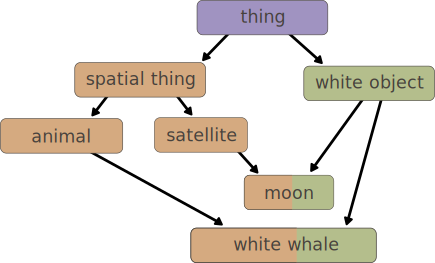
\includegraphics[width=0.6\linewidth]{commonancestors}
        \end{center}

    \only<2>{
\begin{pseudocode}[ruled]{CommonAncestors}{concept1, concept2}
\label{algo|common-ancestors}

\BEGIN
\mathcal{I} \GETS \CALL{Superclasses}{concept1} \cap \CALL{Superclasses}{concept2} \\
\RETURN {c \in \mathcal{I} | \CALL{Subclasses}{c} \cap \mathcal{I} = \emptyset}\\
\END

\end{pseudocode}


    }
    \only<3>{
\begin{pseudocode}[ruled]{FirstDifferentAncestors}{concept1, concept2}
\label{algo|first-different-ancestors}

\BEGIN
\mathcal{C} \GETS \CALL{CommonAncestors}{concept1, concept2} \\
\mathcal{S} \GETS \CALL{Superclasses}{concept1} \cup \CALL{Superclasses}{concept2} \\

\RETURN{\forall c \in \mathcal{C}, \CALL{DirectSubclasses}{c} \cap \mathcal{S}} \\
\END

\end{pseudocode}

    }
\end{frame}


\end{document}
